\section{Specyfikacja techniczna}

\subsection{Architektura systemu}

W obecnie tworzonych systemach spotyka się dwie podstawowe struktury:
architekturę klient-serwer oraz architekturę trójwarstwową.  W
architekturze klient-serwer, która była szczególnie popularna w latach
dziewięćdziesiątych ubiegłego wieku, wyróżnia się dwie warstwy:
\begin{itemize}
\item aplikację użytkownika (\emph{klient});
\item system zarządzania bazą danych (\emph{serwer}).
\end{itemize}

Struktura ta sprawdza się dla prostych systemów, których zadaniem jest
zapisywanie, odczytywanie oraz aktualizacja danych. Problem pojawia
się jednak w przypadku, gdy dane muszą być przetwarzane w nietrywialny
sposób, przy uwzględnieniu dziedziny problemu (ang. \emph{domain
  logic}) modelowanego zagadnienia. Realizacja obliczeń w warstwie
klienta, której głównym zadaniem jest prezentacja informacji
użytkownikowi, może znacząco wpływać na jego komfort pracy oraz
powodować problemy związane z duplikacją kodu źródłowego aplikacji.
Natomiast umieszczenie logiki aplikacji po stronie serwera bardzo
często narzuca przygotowanie programu w środowisku specyficznym dla
danego systemu zarządzania bazami danych.

Problemy te zmusiły projektantów aplikacji do wydzielenia jeszcze
jednego poziomu, który jest odpowiedzialny za logikę operacji na
danych. W architekturze trójwarstwowej uwzględnione są następujące
warstwy:
\begin{itemize}
\item warstwa prezentacji;
\item warstwa aplikacji;
\item warstwa źródła danych.
\end{itemize}

\begin{figure}[h]
  \begin{center}
    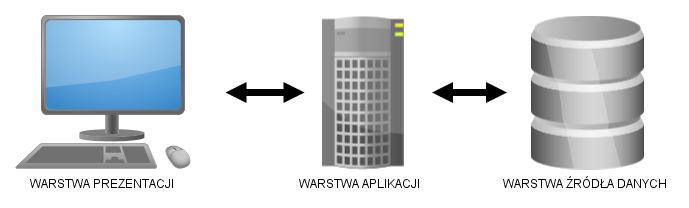
\includegraphics[scale=0.5]{../img/arch-3warstw.png}
  \end{center}
  \label{fig:arch3warstw}
  \caption{Schemat architektury trójwarstwowej}
\end{figure}
\FloatBarrier

W przypadku realizowanego systemu do obsługi magazynu zastosowana
będzie architektura trójwarstwowa.

Na warstwę prezentacji realizowanego systemu składa się:
\begin{itemize}
\item okienkowy interfejs użytkownika (dla kierownika oraz
  magazyniera);
\item serwis webowy (dla sprzedawcy).
\end{itemize}
Warstwa prezentacji komunikuje się z aplikacją w celu wykonania
określonej operacji. Warstwa aplikacji składa się z:
\begin{itemize}
\item warstwy usługowej (serwisów), które są odpowiedzialne za
  wykonywanie niezbędnych operacji (obliczeń, sprawdzania poprawności
  danych wejściowych itp.);
\item warstwy dostępu do danych (DAO).
\end{itemize}

Podstawę całego systemu stanowi relacyjna baza danych.  Schematy bazy
danych opracowany został na podstawie modelu
analitycznego. Przygotowane zostały również perspektywy udostępniające
aplikacji tylko niezbędne informacje.

Podział systemu na komponenty został zaprezentowany na diagramie
\ref{fig:Architektura}.

\begin{figure}[p]
  \begin{center}
    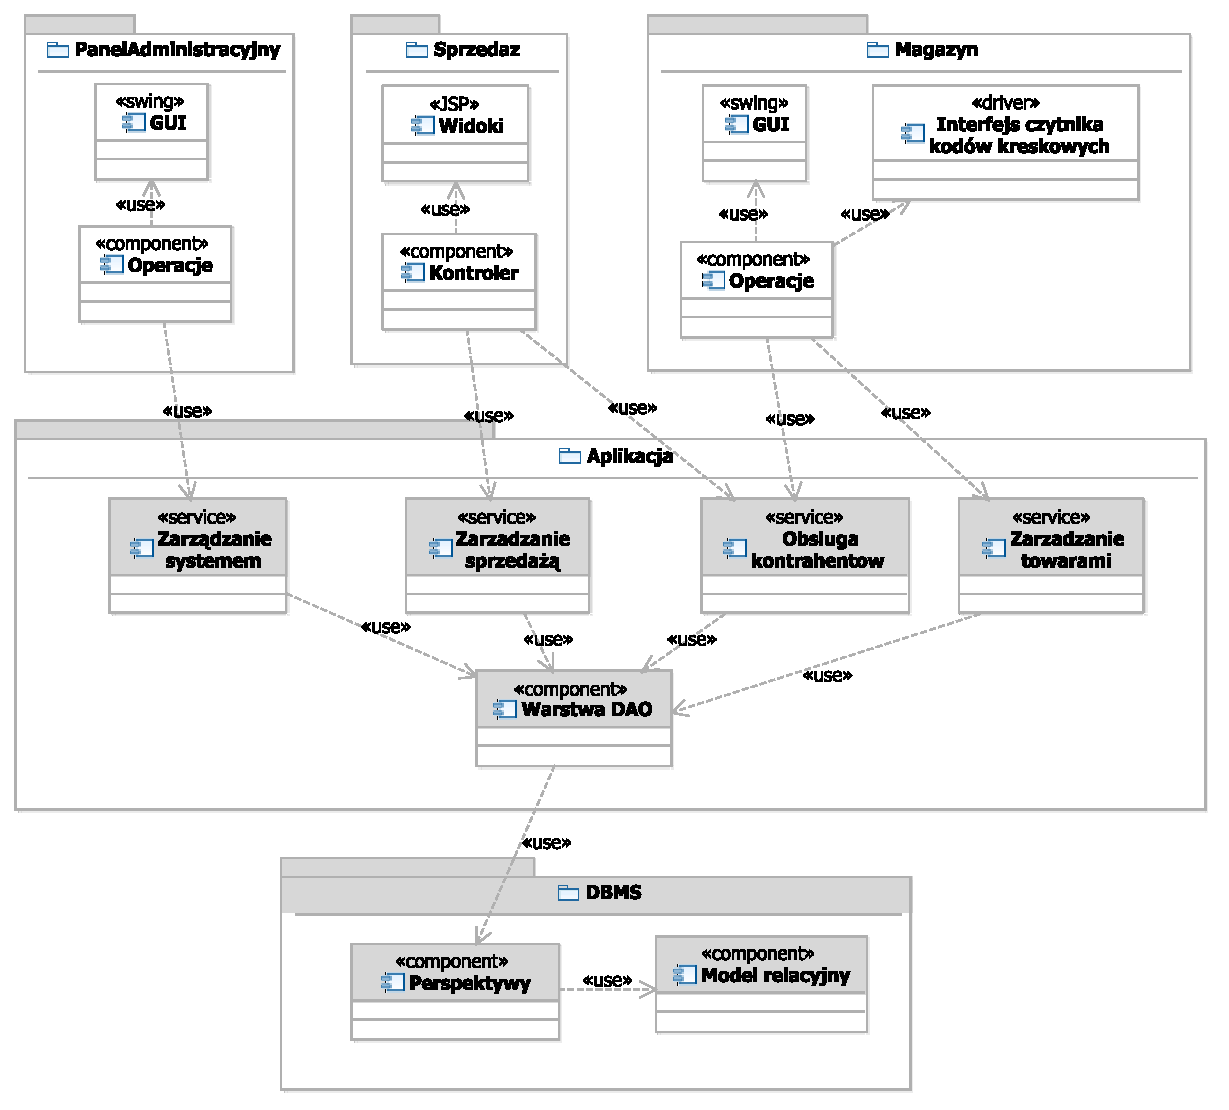
\includegraphics[scale=0.7]{../img/sys/Architektura.pdf}
  \end{center}
  \caption{Architektura systemu}
  \label{fig:Architektura}
\end{figure}
\FloatBarrier

System do magazynowania zostanie przygotowany do pracy w środowisku
maszyny wirtualnej Java. Implementacja zostanie zrealizowana (w
większości) przy użyciu języka Java. Wykorzystane będą następujące
narzędzia:
\begin{itemize}
\item Oracle Swing - w celu implementacji interfejsu użytkownika --
  panelu administracyjnego oraz stanowiska magazyniera;
\item Spring Framework -- biblioteka ta pozwoli na opracowanie
  szkieletu aplikacji realizowanego systemu, w szczególności:
  \begin{itemize}
  \item Spring Remoting -- w celu komunikacji między aplikacją a
    warstwą prezentacji oraz kontenerem webowym;
  \item Spring MVC + widoki JSP w celu implementacji interfejsu
    użytkownika dla sprzedawcy;
  \item Spring Data - w celu uproszczenia implementacji dostępu do
    danych.
  \end{itemize}
\item Hibernate -- w celu komunikacji z warstwą perzystentną.
\end{itemize}

\subsection{Sprzęt i oprogramowanie}

Opracowany system musi być dostępny dla użytkowników spełniających
różne role w przedsiębiorstwie.  W szczególności:
\begin{itemize}
\item kierownik systemu musi mieć dostęp do panelu administracyjnego z
  poziomu sieci lokalnej przedsiębiorstwa (dostęp zewnętrzny do panelu
  administracyjnego ma być uniemożliwiony ze względu na bezpieczeństwo
  danych pracowników);
\item sprzedawca ma mieć dostęp do systemu przy użyciu sieci Internet;
\item magazynier ma mieć dostęp do systemu tylko przy użyciu
  specjalnie przygotowanego dla niego stanowiska.
\end{itemize}

Na diagramie \ref{fig:DiagramWdrozenia} przedstawiono propozycję
wdrożenia systemu.

\begin{figure}[p]
  \begin{center}
    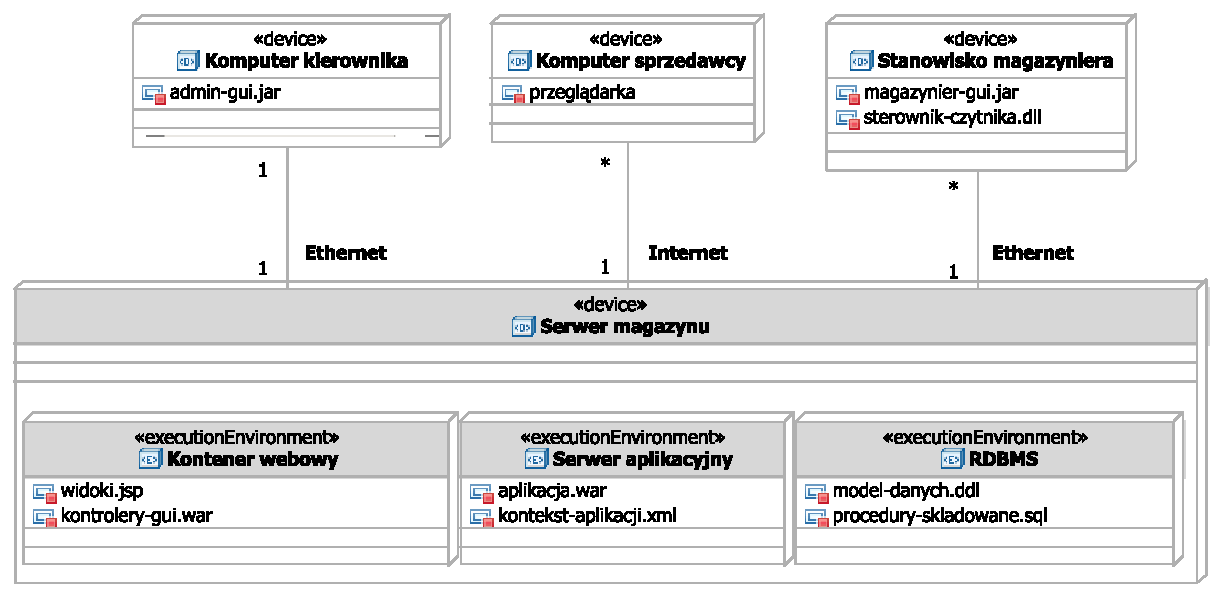
\includegraphics[scale=0.7]{../img/sys/DiagramWdrozenia.pdf}
  \end{center}
  \caption{Propozycja wdrożenia systemu}
  \label{fig:DiagramWdrozenia}
\end{figure}
\FloatBarrier

W poniższych punktach przedstawiono wstępną specyfikację sprzętu i
oprogramowania podstawowego.

\subsubsection{Sprzęt}

\begin{enumerate}
\item Serwer magazynu:
  \begin{itemize}
  \item procesor: 2 x Intel Xeon E5-2620 (2 GHz) 1333MHz;
  \item pamięć: 16 GB LP RDIMM;
  \item dyski twarde: 3 x 300GB (dla standardu Serial Attached SCSI
    (SAS)).
  \end{itemize}
\item Stanowisko magazyniera:
  \begin{itemize}
  \item komputer stacjonarny:
    \begin{itemize}
    \item procesor: Intel Core i5-3470;
    \item pamięć: 4GB DDR3-1333;
    \item pojemność dysku: 200GB;
    \end{itemize}
  \item czytnik kodów kreskowych Motorola LS2208.
  \item drukarka igłowa OKI ML 3321
  \end{itemize}
\end{enumerate}

\subsubsection{Oprogramowanie}

\begin{enumerate}
\item Serwer magazynu:
  \begin{itemize}
  \item stabilna wersja systemu Debian (obecnie 7.0 \emph{Wheezy});
  \item serwer aplikacyjny oraz kontener webowy: Apache Tomcat 7.0.40; uruchamiane dla Oracle JVM 1.7;
  \item relacyjna baza danych PostgreSQL 9.2.4.
  \end{itemize}
\item Stanowisko magazyniera:
  \begin{itemize}
  \item system operacyjny Microsoft Windows 7;
  \item Oracle JVM 1.7;
  \item sterowniki dostępne dla czytnika kodów kreskowych Motorola LS2208.
  \item sterowniki producenta dla drukarki igłowej OKI ML 3321
  \end{itemize}
\end{enumerate}

Opracowana aplikacja dostępowa -- panel administracyjna będzie działać dla:
\begin{itemize}
\item Microsoft Windows XP, Vista, 7, 8;
\item Linux/Unix dla jądra systemu o wersji powyżej 3.2.
\end{itemize}
W obu przypadkach wymagana jest instalacja Oracle JVM 1.7.

Opracowana aplikacja dostępowa dla sprzedawcy będzie działać dla systemów
wyposażonych w przeglądarki internetowe:
\begin{itemize}
\item Mozilla Firefox dla wersji powyżej 3.6;
\item Google Chrome dla wersji powyżej 26.0;
\item Opera dla wersji powyżej 11.0;
\item Internet Explorer dla wersji powyżej 10.
\end{itemize}


